\subsection{Rule based Overtake}\label{s:testRuleOvertake}
    \paragraph{Scenario:} Two UAS are flying in the \emph{controlled airspace} (over 500 feet Above Ground Level) on the \emph{airway} (in same direction). \emph{Slower UAS} is in front of \emph{Faster UAS}. There is possibility of a \emph{collision} or a \emph{near miss incident} or a \emph{well clear breach}. The \emph{Faster UAS} (Overtaking) must contact \emph{UTM} service and ask for \emph{overtake permission}. Scenario steps:
    
    \begin{enumerate}
        \item \emph{Faster UAS} (Overtaking) notices \emph{UTM} service about \emph{Slower UAS} (Overtaken). (This step is Optional.)
        
        \item \emph{UTM} service issues \emph{Directives} to all \emph{UAS} in area.
        
        \item \emph{Overtake Directive} is received by \emph{Faster UAS} (Overtaking) and \emph{Slower UAS} (Overtaken).
        
        \item \emph{Faster UAS} (Overtaking) mission plan is altered to reflect \emph{Overtake directive}, \emph{Divergence Waypoint} and \emph{Convergence Waypoint} are added.
        
        \item \emph{Faster UAS} (Overtaking) safely overtakes \emph{Slower UAS} (Overtaken) without breaking \emph{Well clear} condition.
    \end{enumerate}
    
    \noindent\emph{Mission parameters} for both \emph{UAS} systems are defined in (tab. \ref{tab:missionSetupRuleBasedOvertakeScenarios}).
    
    \begin{table}[H]
        \centering
        \begin{tabular}{c||c|c||c}
            \multirow{2}{*}{UAS} &\multicolumn{2}{c||}{Position} & \multirow{2}{*}{$\mathscr{WP}_1$} \\\cline{2-3}
              & $[x,y,z]$           & $[\theta,\varpi,\psi]$           & \\\hline\hline
            1 & $[-40,20,0]^T $       & $[0^\circ,0^\circ,0^\circ]^T$    & $[110,20,0]^T$\\\hline 
            2 & $[-20,20,0]^T $       & $[0^\circ,0^\circ,0^\circ]^T$    & $[80,20,0]^T$\\
        \end{tabular}
        \caption{Mission setup for all \emph{Rule based overtake} scenarios.}
        \label{tab:missionSetupRuleBasedOvertakeScenarios}
    \end{table}


    \paragraph{Assumptions:} Following assumptions are valid for this test:
    
    \begin{enumerate}
        \item \emph{Controlled Airspace Airworthiness} - UAS system is equipped with necessary controlled airspace equipment like ADS-B In/Out, Radar, Transponder, etc. Moreover airworthy \emph{UAS} has capability to precisely follow \emph{UTM directives} (max. 5 $\%$ deviation).
        
        \item \emph{C2 (Command \& control) Link Established} - necessary for (UAS $\leftrightarrow$ UAS) and (UAS $\leftrightarrow$ UTM) communication. If \emph{C2} link is lost the \emph{UAS} will enter into \emph{Emergency avoidance mode}.
        
        \item \emph{Decision frame synchronization with UTM} - necessary in discrete C2 environment otherwise \emph{safety margins} needs to be \emph{bloated}.
    \end{enumerate}
    
    \paragraph{Main Goal:} Show possibility of \emph{Overtake Maneuver} invoked by the \emph{UTM Directive} (event based flight constraint). 
    
    \paragraph{Acceptance Criteria:} Following criteria must be met:
    \begin{enumerate}
        \item \emph{Proper passing of Divergence/Convergence Waypoint} - minimal distance of \emph{UAS trajectory} to \emph{Divergence/Convergence waypoint} must be below passing threshold. Waypoints needs to be passed in given order (Divergence $1^{st}$, Convergence $2^{nd}$).
        
        \item \emph{Slower UAS (Overtaken) keeps Right of the Way} - the UAS with lesser maneuverability does not stand a chance in avoidance situation, it needs to keep its \emph{Right of the Way}. 
        
        \item \emph{Both UAS does not breach Well Clear (safety) Margin} - mutual distance does not get trough \emph{calculated Safety Margin}.
    \end{enumerate}
    
    \paragraph{Testing Setup:} The \emph{standard test setup} for each UAS defined in (tab. \ref{tab:testMovementOrientations}, \ref{tab:testUASBasicParameters}, \ref{tab:testNavigationGridBasic}, \ref{tab:testAvoidanceGridBasic}, \ref{tab:testUASColoring}) is used with following parameter override:
    \begin{enumerate}
        \item \emph{Navigation grid - type} - \emph{ACAS-like} with enabled \emph{Horizontal maneuvers}
    \end{enumerate}
    
    This \emph{configuration} is based on assumption that every UAS is in \emph{controlled airspace} in \emph{FL450} (flight level 45000 feet Above Sea Level), without permission for \emph{climb or descent maneuver}. \emph{Rule engine} is initialized in standard \emph{Rules of the air} configuration (fig. \ref{fig:RuleEngineInstanceLevels}).
    
    There is \emph{UTM} service for given \emph{airspace cluster} calculating \emph{collision cases} (tab. \ref{tab:collisionCase}) based on incoming \emph{UAS position notifications} (tab. \ref{tab:positionNotification}).
    
    
    \paragraph{Simulation Run:} Notable moments from the \emph{simulation run} (fig. \ref{fig:testCaseRuleBasedOvertake2xSpeed}) are following:
    
    \begin{enumerate}
        \item \emph{Collision case creation} (fig.\ref{fig:ruleBasedOvertake2xCollisionCaseCreation}) - \emph{Faster UAS} (blue) receives \emph{UTM Directive} to invoke \emph{Overtake Rule} (tab. \ref{tab:ruleOvertakeDefinition}). \emph{Slower UAS} (magenta) receives \emph{UTM Directive} to keep \emph{Right of the Way} and warning that is going to be \emph{Overtaken}. \emph{Faster UAS} (blue) creates two \emph{virtual waypoints}:
        \begin{enumerate}[a.]
            \item \emph{Divergence waypoint} at position $[0,14,0]^T$.
            \item \emph{Convergence waypoint} at position $[24,14,0]^T$.
        \end{enumerate}
        \emph{Faster UAS} then sets \emph{Divergence waypoint} as \emph{Goal waypoint} and It starts overtake maneuver while checking mutual distance.
        
        \item \emph{Divergence waypoint reach} (fig. \ref{fig:ruleBasedOvertake2xDivergenceWaypointReach}) - \emph{Faster UAS} (blue) successfully reached \emph{Divergence Waypoint}, setting \emph{Convergence Waypoint} as new \emph{Goal waypoint}.
        
        \item \emph{Convergence waypoint reach} (fig. \ref{fig:ruleBasedOvertake2xConvergenceWaypointReach}) - \emph{Faster UAS} (blue) successfully reached \emph{Convergence Waypoint}, setting \emph{Original Goal Waypoint} as new \emph{Goal waypoint}. The \emph{UTM} service is notified from \emph{Faster UAS} (blue) that \emph{Overtaken Maneuver} have been completed. UTM \emph{acknowledges} maneuver competition and It sends notification to \emph{Slower UAS} (magenta) that \emph{Overtake Maneuver} is finished. \emph{Slower UAS} (magenta) was successfully overtaken.
        
        \item \emph{Original waypoint reach} (fig. \ref{fig:ruleBasedOvertake2xOriginalWaypointReach}) - \emph{Faster UAS} (blue) successfully reached \emph{Original Waypoint}, Starting landing Sequence. 
    \end{enumerate}


    \begin{figure}[H]
        \centering
        \begin{subfigure}{0.75\textwidth}
            \centering
            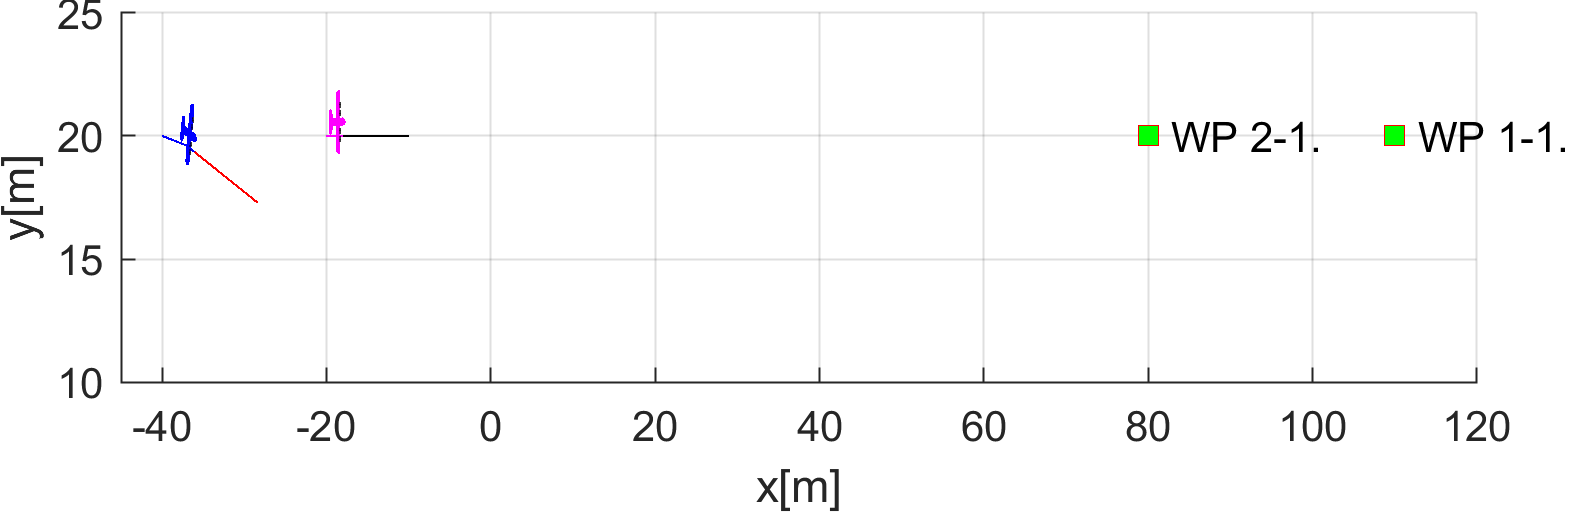
\includegraphics[width=0.9\linewidth]{\FIGDIR/NS071UtmCooperativeOvertake2xSpeed00002}
            \caption{Collision case creation.}
            \label{fig:ruleBasedOvertake2xCollisionCaseCreation}
        \end{subfigure}
        \\
        \begin{subfigure}{0.75\textwidth}
            \centering
            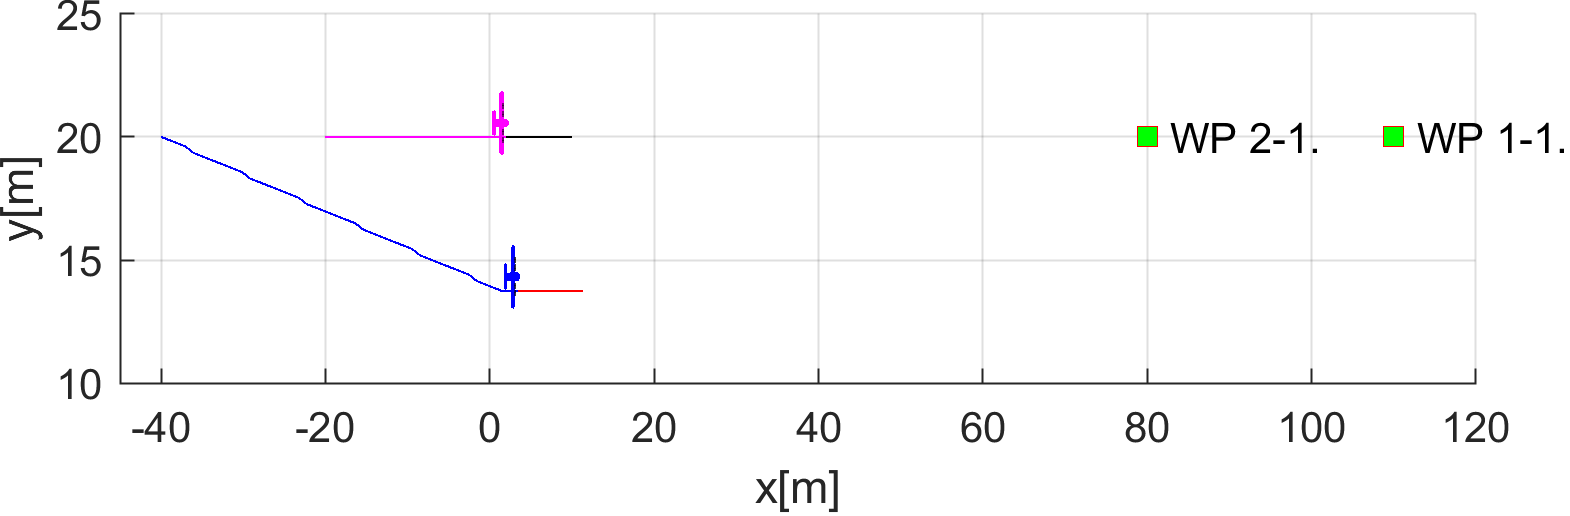
\includegraphics[width=0.9\linewidth]{\FIGDIR/NS072UtmCooperativeOvertake2xSpeed00022} 
            \caption{Divergence waypoint reach.}
            \label{fig:ruleBasedOvertake2xDivergenceWaypointReach}
        \end{subfigure}
        \\
        \begin{subfigure}{0.75\textwidth}
            \centering
            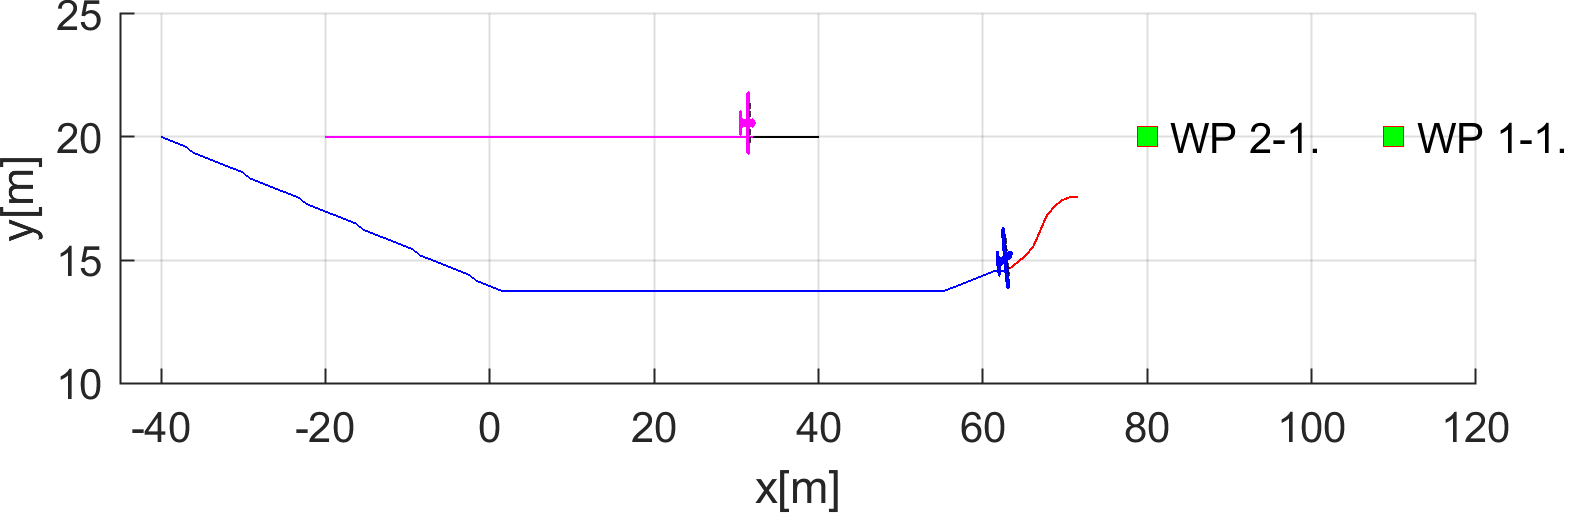
\includegraphics[width=0.9\linewidth]{\FIGDIR/NS073UtmCooperativeOvertake2xSpeed00052} 
            \caption{Convergence waypoint reach.}
            \label{fig:ruleBasedOvertake2xConvergenceWaypointReach}
        \end{subfigure}
        \\
        \begin{subfigure}{0.75\textwidth}
            \centering
            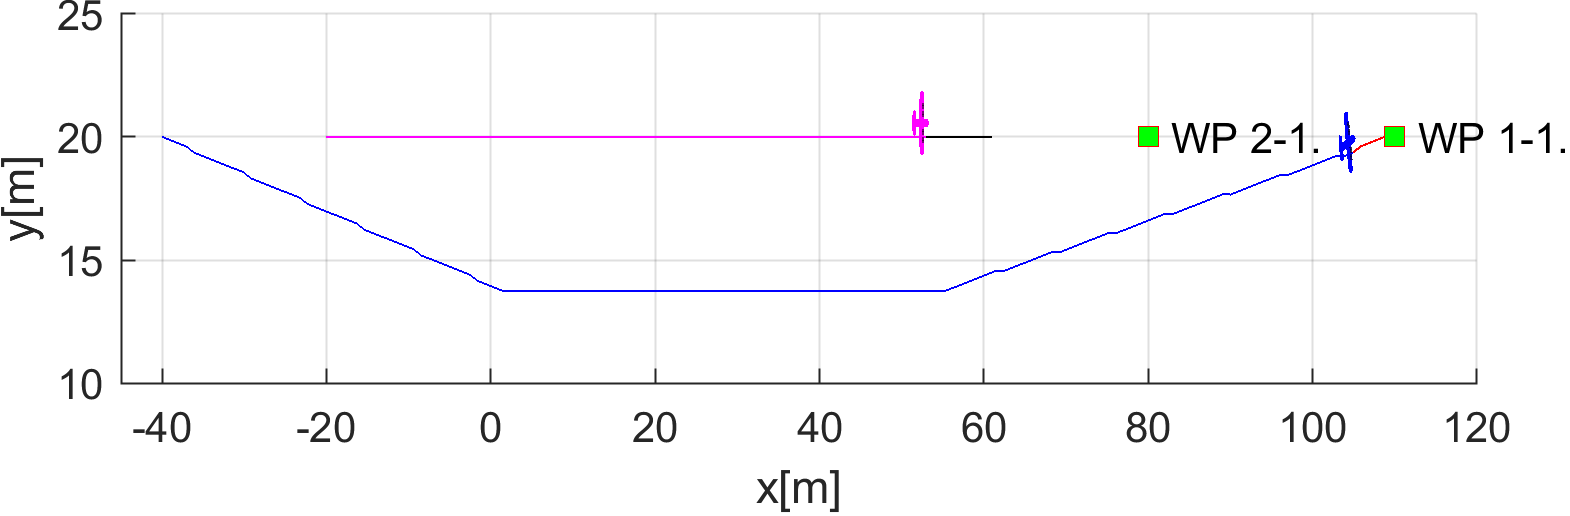
\includegraphics[width=0.9\linewidth]{\FIGDIR/NS074UtmCooperativeOvertake2xSpeed00073} 
            \caption{Original waypoint reach.}
            \label{fig:ruleBasedOvertake2xOriginalWaypointReach}
        \end{subfigure}
        \caption{Test scenario for \emph{Rule based Overtake} (double speed of overtaking aircraft). }
        \label{fig:testCaseRuleBasedOvertake2xSpeed}
    \end{figure}
    

    \paragraph{Collision Case Calculation:} The \emph{Collision Case} (tab. \ref{tab:collisionCasesRuleOvertake2x}) was calculated according to \emph{Collision Calculation process} (sec. \ref{sec:collisionCase}). \emph{Faster UAS} (1) has \emph{Overtaking} role and \emph{Slower UAS} has \emph{Right of the Way}. \emph{Collision Point} is direct type at $[0.20.0]^T$. \emph{Collision case type} was set based on \emph{angle of approach} $0^{\circ}$ as \emph{Overtake}. The \emph{Safety Margin} was set as \emph{5 m}.
    
    
    \begin{table}[H]
        \centering
        \begin{tabular}{c|c|c|c|c|c||c|c}
            \multicolumn{6}{c||}{Collision Case}& \multicolumn{2}{c}{Margins} \\ \hline
            id  & UAS & role & \begin{tabular}[c]{@{}c@{}}collision\\ point\end{tabular} & \begin{tabular}[c]{@{}c@{}}angle of\\ approach\end{tabular} & type&  safety  & case  \\ \hline\hline
            % Case 1-2
            \multirow{2}{*}{1-2} & 1   & Overtaking & \multirow{2}{*}{$[0,20,0]^T$} & \multirow{2}{*}{$0^\circ$} & \multirow{2}{*}{Overtake} & 5 & \multirow{2}{*}{5} \\ \cline{2-3} \cline{7-7} & 2   & Right o.W. & & & & 5& \\ 
        \end{tabular}
        \caption{Collision case for \emph{Rule-based Overtake} scenario 2x speed.}
        \label{tab:collisionCasesRuleOvertake2x}
    \end{table}
    
    
    \paragraph{Overtake Speed: Divergence/Convergence Waypoints}
    \emph{Divergence waypoints} have been calculated according to (eq. \ref{eq:overtakeDivergenceLocal}), and, \emph{Convergence Waypoints} have been calculated according to (eq. \ref{eq:overtakeConvergenceLocal}). Following \emph{Speed Differences} were taken into account (Faster/Slower UAS speed ratio): \emph{2x, 3x, 4x}. Following observations can be made:
    
    \begin{enumerate}
        \item \emph{Distance between Divergence and Convergence waypoint} is decreasing with increasing \emph{speed difference}.
        
        \item \emph{Divergence waypoint} is moving \emph{back/right} in \emph{UAS Local Coordinate Frame} with Increasing \emph{speed difference}. 
        
        \item \emph{Convergence waypoint} is moving like \emph{Divergence waypoint} but little bit faster.
    \end{enumerate}
    
    \begin{table}[H]
        \centering
        \begin{tabular}{c||c|c||c|c||c}
            %Header line 1
            \multirow{2}{*}{\begin{tabular}[c]{@{}c@{}}Speed\\ diff.\end{tabular}} & \multicolumn{2}{c||}{Divergence} & \multicolumn{2}{c||}{Convergence} & \multirow{2}{*}{\begin{tabular}[c]{@{}c@{}}Final\\ waypoint\end{tabular}} \\ \cline{2-5}
            %Header line 2
            & waypoint & \multirow{2}{*}{difference} & waypoint & \multirow{2}{*}{difference}  & \\ \cline{1-2} \cline{4-4} \cline{6-6} 
            % 2x speed 
            \multirow{2}{*}{2x} & \multirow{2}{*}{$[0,14,0]^T$} & & \multirow{2}{*}{$[24,14,0]^T$} & & \multirow{2}{*}{$[110,20,0]^T$} \\ \cline{3-3} \cline{5-5} 
            %  2-3 diff
            & & \multirow{2}{*}{$[-10,-1,0]^T$} & & \multirow{2}{*}{$[-8,-1,0]^T$} & \\ \cline{1-2} \cline{4-4} \cline{6-6} 
            % 3x speed
            \multirow{2}{*}{3x} & \multirow{2}{*}{$[-10,13,0]^T$} & & \multirow{2}{*}{$[16,13,0]^T$} & & \multirow{2}{*}{$[110,20,0]^T$} \\ \cline{3-3} \cline{5-5}
            % 3-4 diff
            & & \multirow{2}{*}{$[-3.4,-1,0]^T$} & & \multirow{2}{*}{$[-1.3,-1,0]^T$} & \\ \cline{1-2} \cline{4-4} \cline{6-6} 
            % 4x speed
            \multirow{2}{*}{4x} & \multirow{2}{*}{$[-13.4,12,0]^T$} & & \multirow{2}{*}{$[14.7,12,0]^T$} & & \multirow{2}{*}{$[110,20,0]^T$} \\ \cline{3-3} \cline{5-5}
            %filler line
            & & & & & \\ 
            \end{tabular}
        \caption{Convergence and divergence waypoints for various speed differences.}
        \label{tab:convergenceDivergenceWaypointsOvertake}
    \end{table}
    
    \paragraph{Overtake Speed: Impact on Trajectory} Overtake \emph{speed difference} is visible in (fig. \ref{fig:testCaseRuleBasedOvertakeDifferentSpeedTrajectoriesPerformance}). The \emph{Slower vehicle trajectory}(cyan) is following \emph{standard mission waypoints}. The \emph{Faster vehicle trajectory} for 2x (blue), 3x (green), 4x (black) are following \emph{Divergence/Convergence} waypoints from (tab. \ref{tab:convergenceDivergenceWaypointsOvertake}).
    
    \begin{figure}[H]
        \centering
        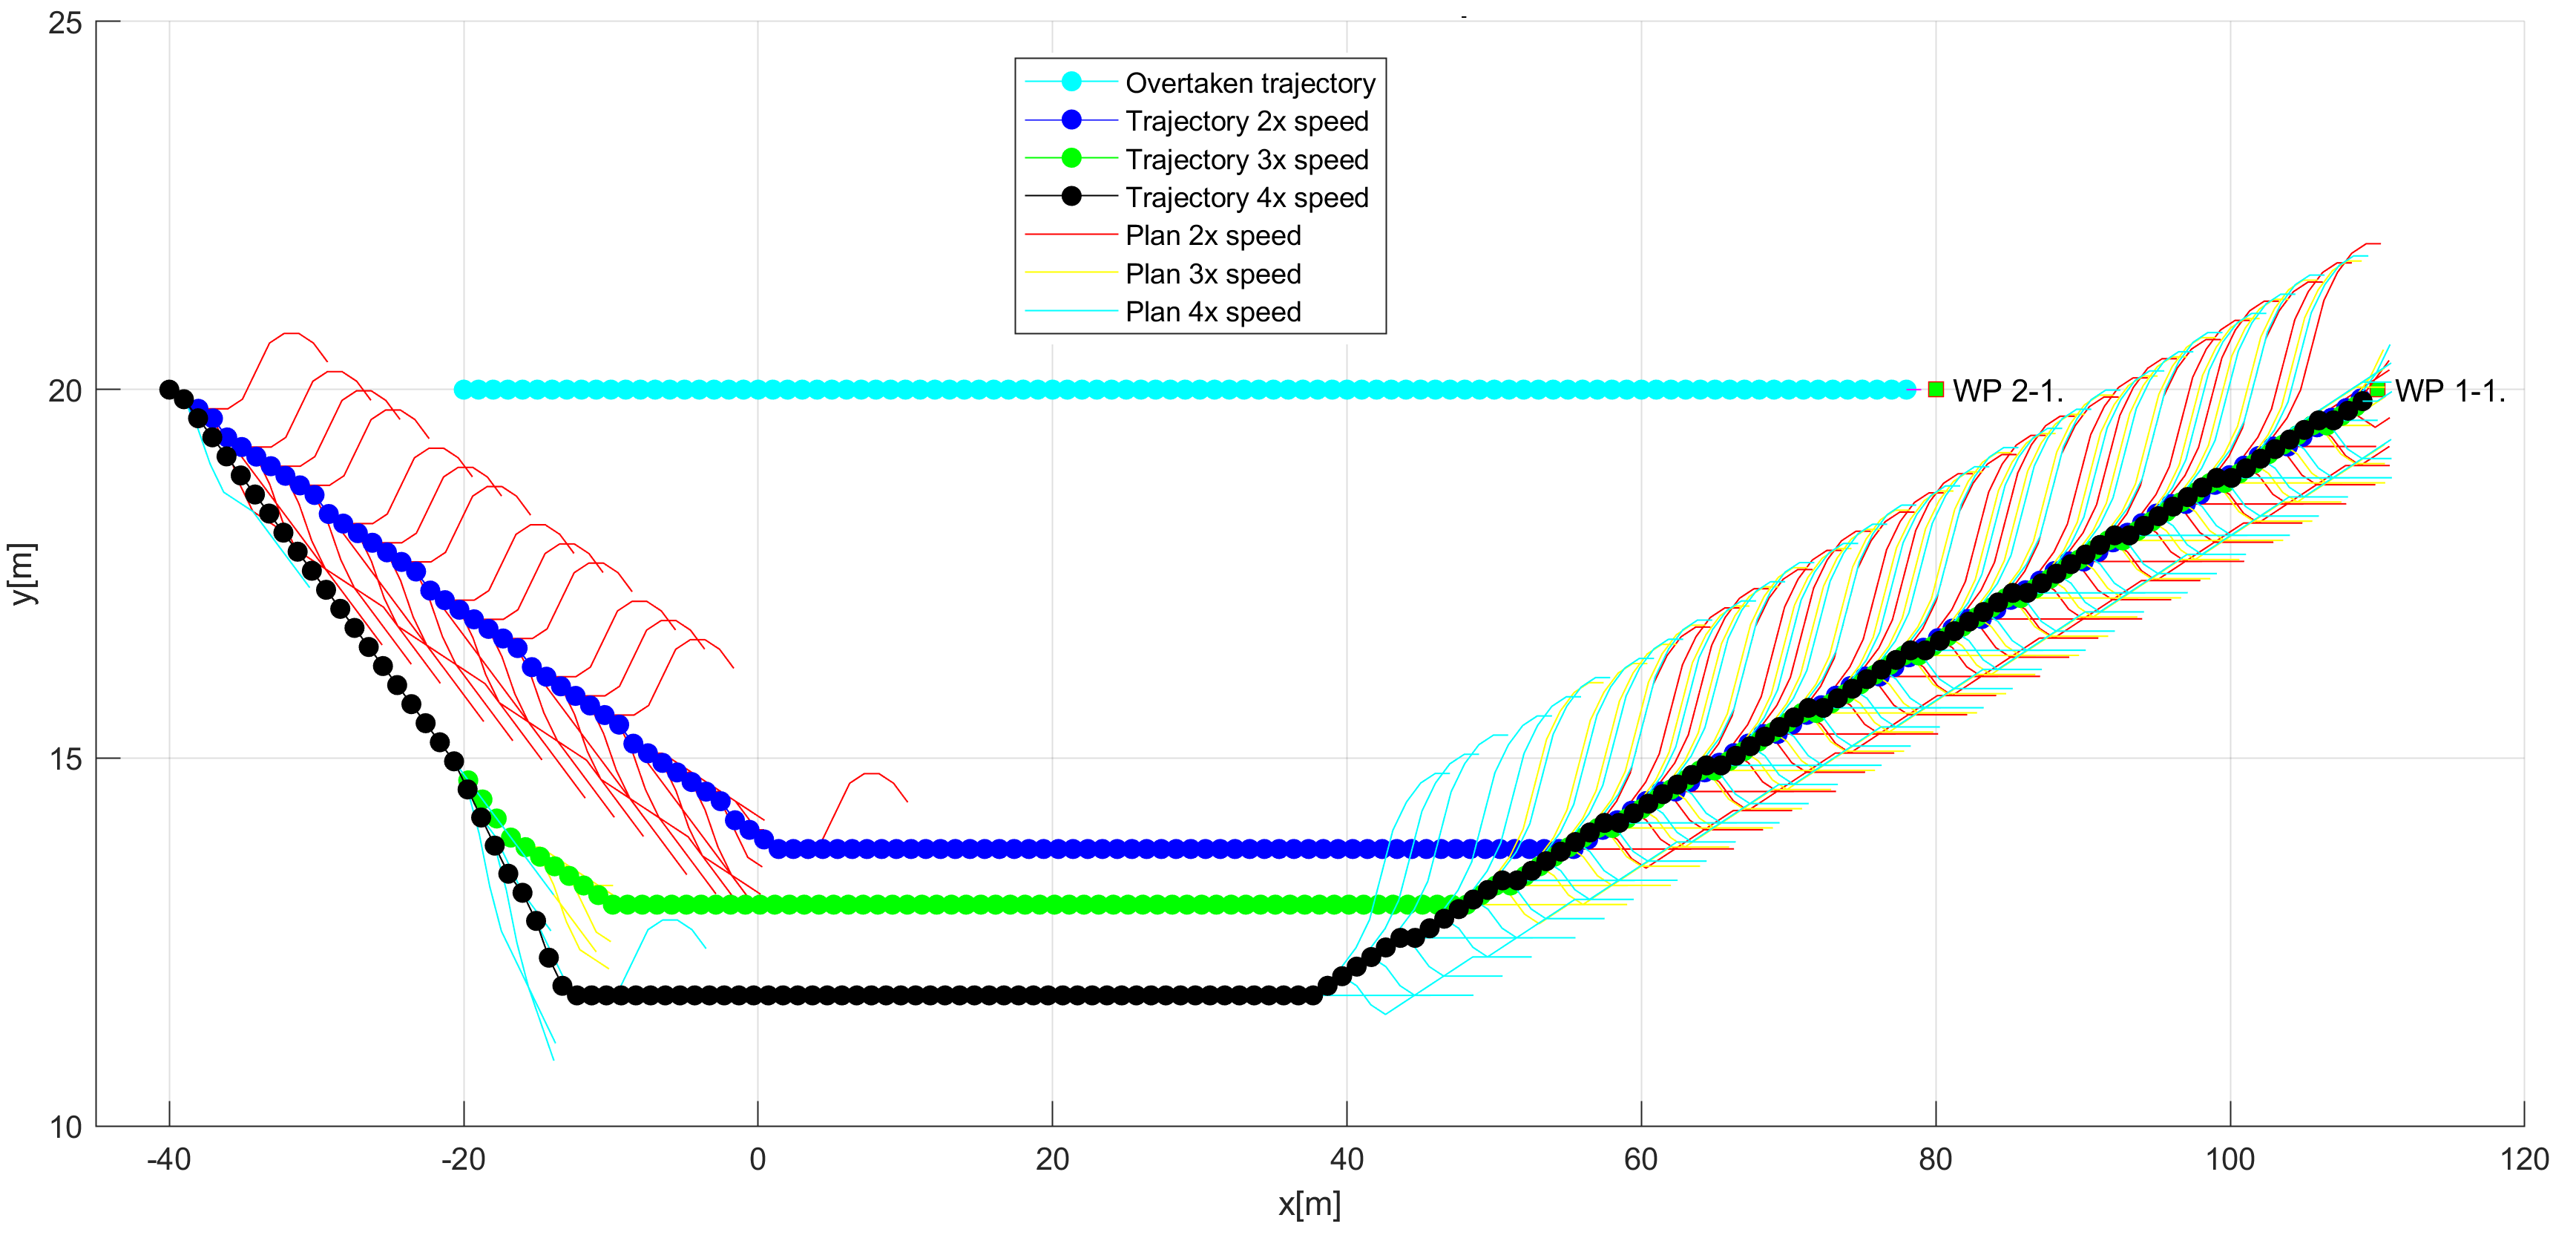
\includegraphics[width=0.9\linewidth]{\FIGDIR/NS078UtmCooperativeOvertakeMultipleTrajectories}
        \caption{\emph{Rule based overtake} trajectories for different speed.}
        \label{fig:testCaseRuleBasedOvertakeDifferentSpeedTrajectoriesPerformance}
    \end{figure}
    
    \paragraph{Overtake Speed: Impact on Distance to Safety Margin Evolution} \emph{Safety margin} (red line) is set to \emph{5 m}. It is obvious that \emph{Faster UAS} will take down \emph{Slower UAS} if there was not for an \emph{Overtake maneuver}.  The distance of \emph{Faster UAS} to \emph{Slower UAS} evolution is depending on \emph{Speed difference}. \emph{Inflection point} (closest point of two UAS) is reached sooner with \emph{Higher speed}. \emph{Safety margin performance} was measured for the \emph{UTM performance time} in interval $[0,35]$ $s$ and \emph{Speed difference} of 2x (blue), 3x (green), 4x (black).
    
    \begin{figure}[H]
        \centering
        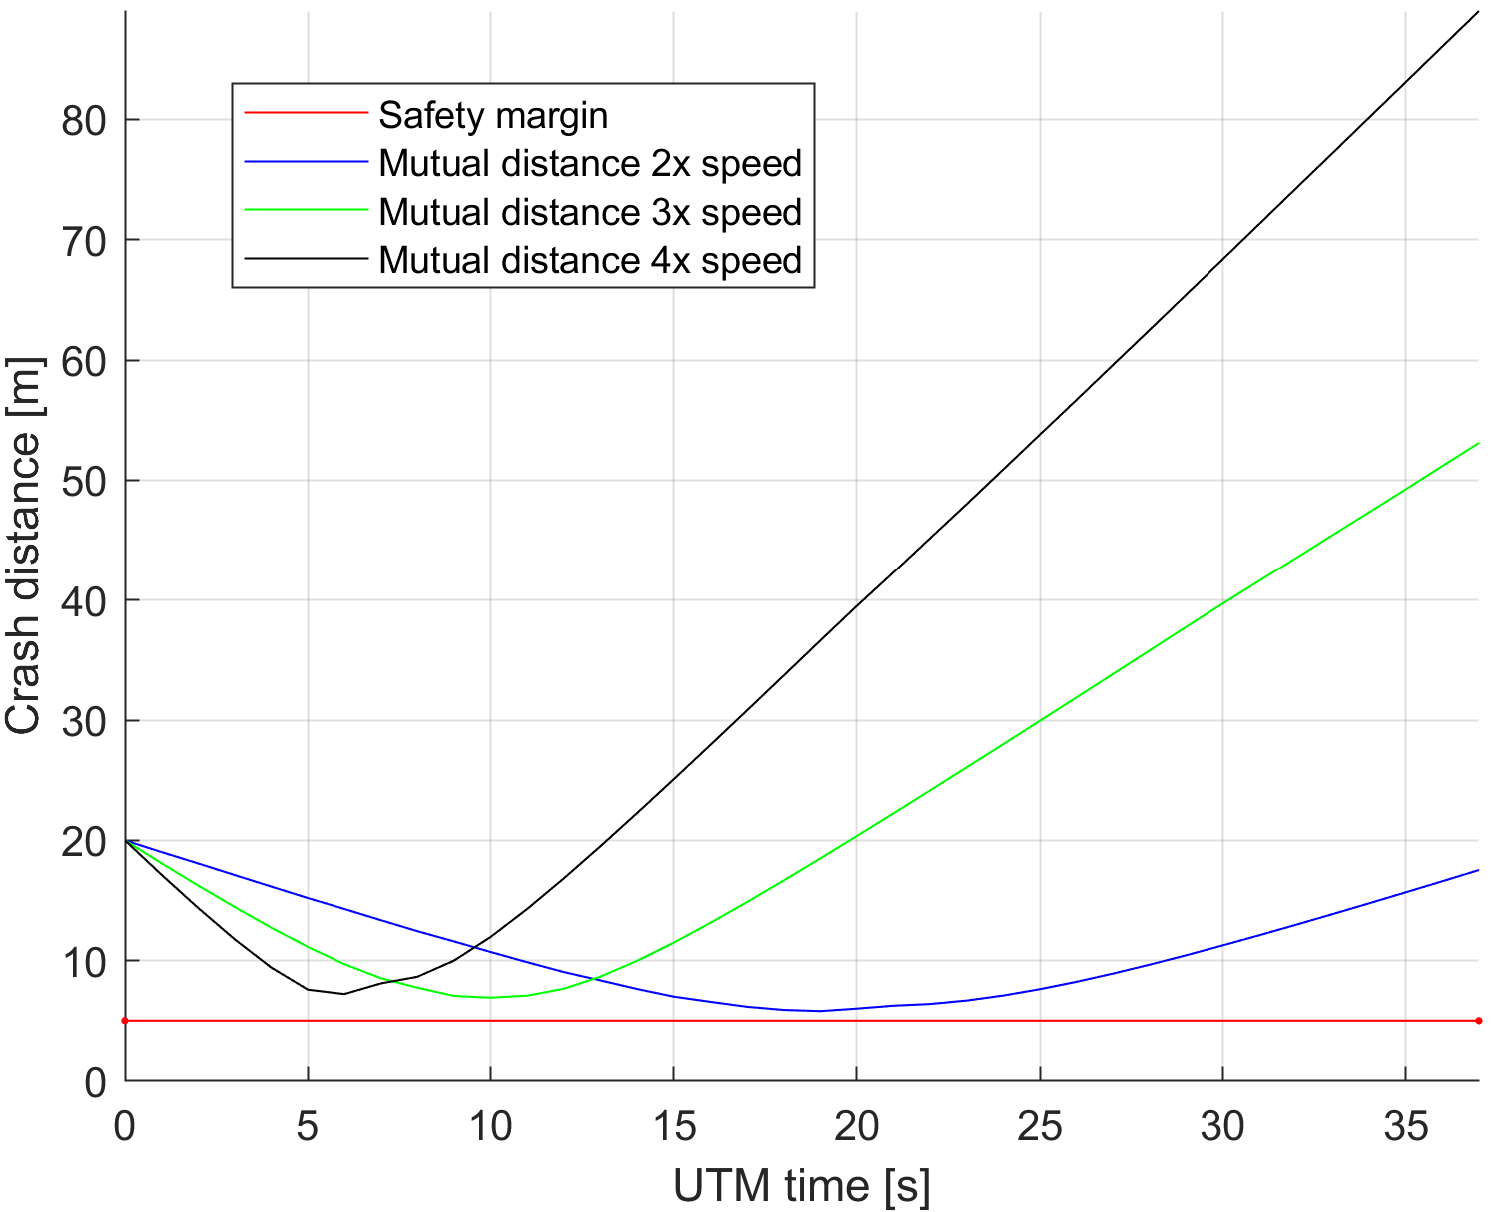
\includegraphics[width=0.6\linewidth]{\FIGDIR/NS079UtmCooperativeOvertakeMultiplePerformance}
        \caption{Overtake speed dependent distance to safety margin evolution for \emph{rule based overtake scenario}.}
        \label{fig:testRuleBasedOvertakeSafetyMarginForDifferentSpeedPerformance}
    \end{figure}
    
    \paragraph{Overtake Speed: Impact on Distance to Safety Margin Peaks} There is summary table (tab. \ref{tab:testCaseRuleBasedOvertakeSafetyMarginDistancesTimes}) for  measurement of minimal and maximal values for \emph{Distance to Safety Margin} over \emph{UTM time} (fig.\ref{fig:testRuleBasedOvertakeSafetyMarginForDifferentSpeedPerformance}). The minimal \emph{Overtake Distance to Safety Margin} in $0.7991$ $m$ for 2x \emph{Speed Difference}. The minimal \emph{Overtake closest point reach time} is $7$ $s$ for 4x \emph{Speed Difference}.
    
    For each \emph{Speed difference} (2x, 3x, 4x), the \emph{Well Clear Margin} (Safety Margin) was not reached by the \emph{Faster UAS Body boundary}.  
    
    \begin{table}[H]
        \centering
        \begin{tabular}{c||c|c||c|c||c}
        %Header
        \multirow{2}{*}{\begin{tabular}[c]{@{}c@{}}Speed\\ diff.\end{tabular}} & \multicolumn{2}{c||}{Minimal} & \multicolumn{2}{c||}{Maximal} & \multirow{2}{*}{Breach} \\ \cline{2-5}
        %Header2
        & distance & time & distance & time & \\ \hline\hline
        % speed 2x
        2x & 0.7991 & 20 & 48.8508 & 76 & false \\ \hline
        % speed 3x
        3x & 1.9180 & 11 & 73.5336 & 51 & false \\ \hline
        % speed 4x
        4x & 2.2154 & 7 & 84.0721 & 38 & false \\ 
        \end{tabular}
        \caption{Distance to safety margin peaks for various overtake speed in \emph{Rule based overtake scenario}.}
        \label{tab:testCaseRuleBasedOvertakeSafetyMarginDistancesTimes}
    \end{table}
    
    \paragraph{Path Tracking Performance: 2x Speed} Performance was only evaluated for case when \emph{Faster/Slower UAS speed ratio} is $2x$. All waypoints are marked as green numbered \emph{squares} with number. Initial waypoint is marked as green square with \emph{S}. Reference trajectory is annotated as \emph{green dashed line}. \emph{Executed trajectory is annotated} as \emph{blue solid line}.
    
    Following observations can be made from path tracking  (fig. \ref{fig:testCaseRuleBasedOvertake2xTrajectoryTracking}):
    
    \begin{enumerate}
        \item \emph{UAS 2 has the Right of the Way} (fig. \ref{fig:ruleBasedOvertake2xPathTrackingUAS2}) - \emph{reference trajectory} and \emph{executed trajectory} are identical. 
        
        \item \emph{UAS 1 is Overtaking} (fig. \ref{fig:ruleBasedOvertake2xdPathTrackingUAS1}) - the following waypoins are marked on reference trajectory:
        \begin{enumerate}[a.]
            \item \emph{Collision Point} ($\mathscr{WP}$ 1.) - this is not used for navigation, its marking of \emph{Collision Point}.
            \item \emph{Divergence waypoint} ($\mathscr{WP}$ 2.) - there will \emph{Faster UAS} navigate to avoid \emph{Collision}.
            \item \emph{Convergence waypoint} ($\mathscr{WP}$ 3.) - there will \emph{Faster UAS} navigate to gain \emph{Safe Return Distance}.
            \item \emph{Original Goal Waypoint} ($\mathscr{WP}$ 4.) - there will \emph{Faster UAS} continue until \emph{original goal} is reached. 
        \end{enumerate}
    \end{enumerate}
    
    \begin{figure}[H]
        \centering
        \begin{subfigure}{0.48\textwidth}
        	\centering
            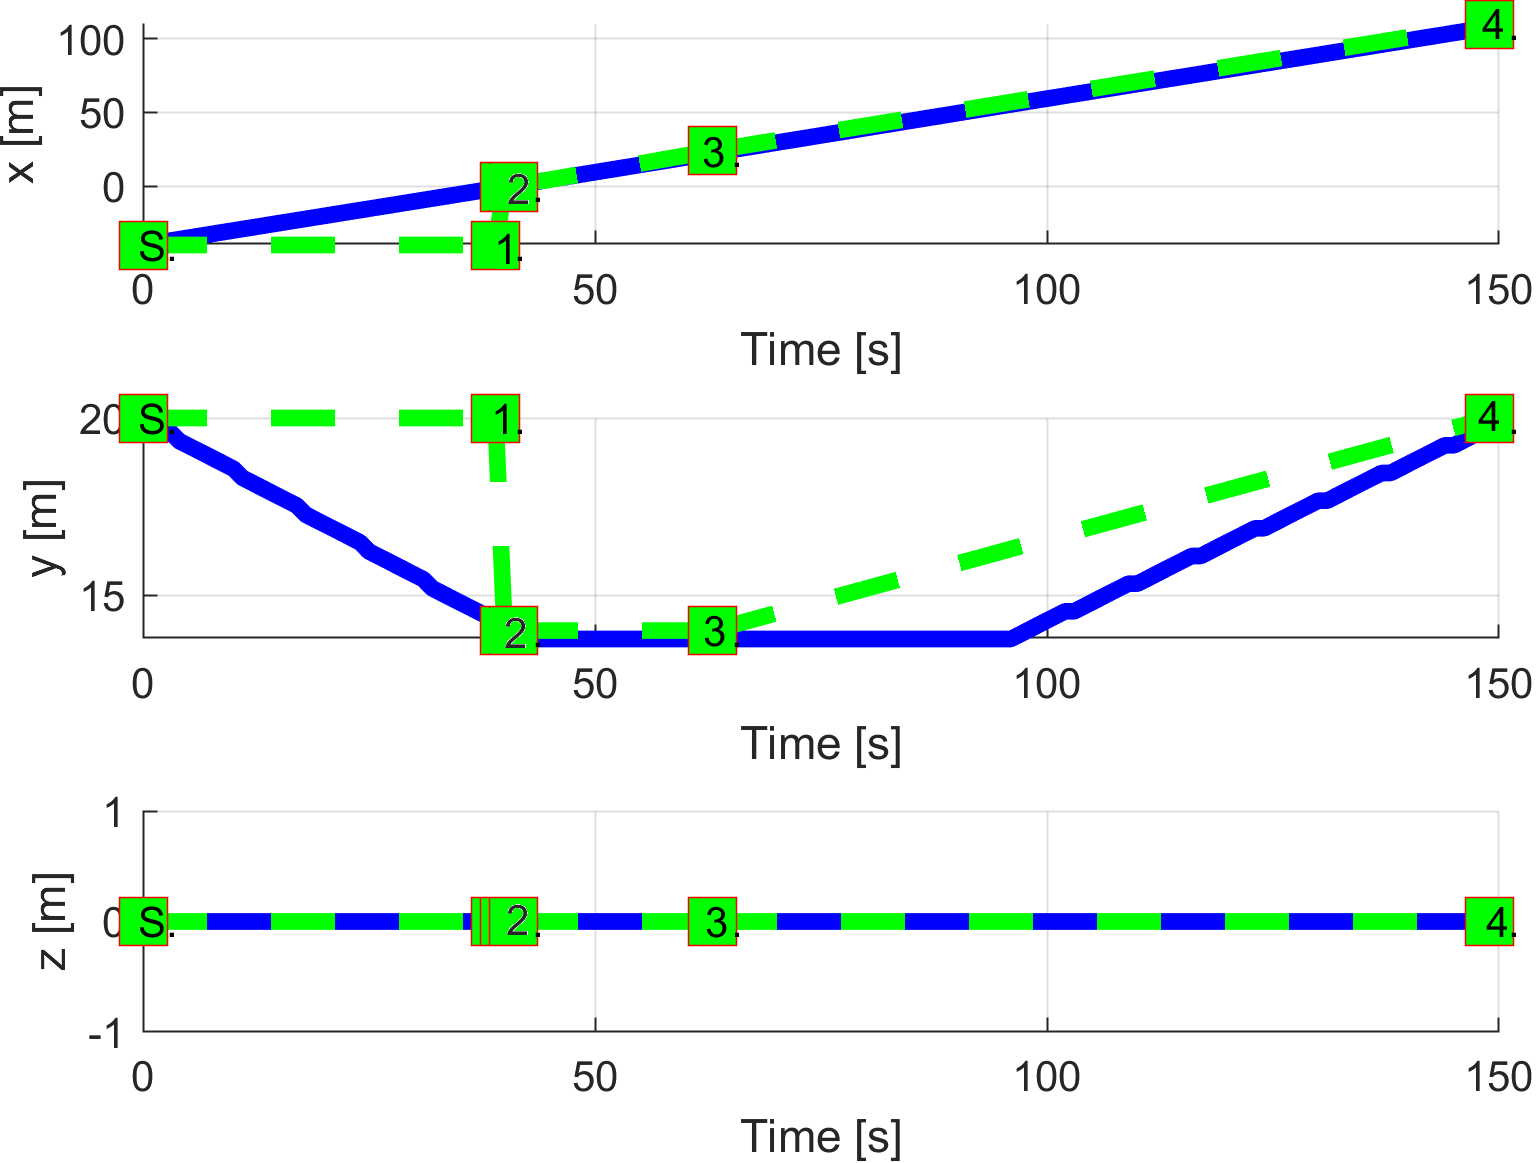
\includegraphics[width=0.9\linewidth]{\FIGDIR/NS076UtmCooperativeOvertake2xSpeedUAV1PathFollowing}
            \caption{UAS 1.}
            \label{fig:ruleBasedOvertake2xdPathTrackingUAS1}
        \end{subfigure}
        \begin{subfigure}{0.48\textwidth}
        	\centering
            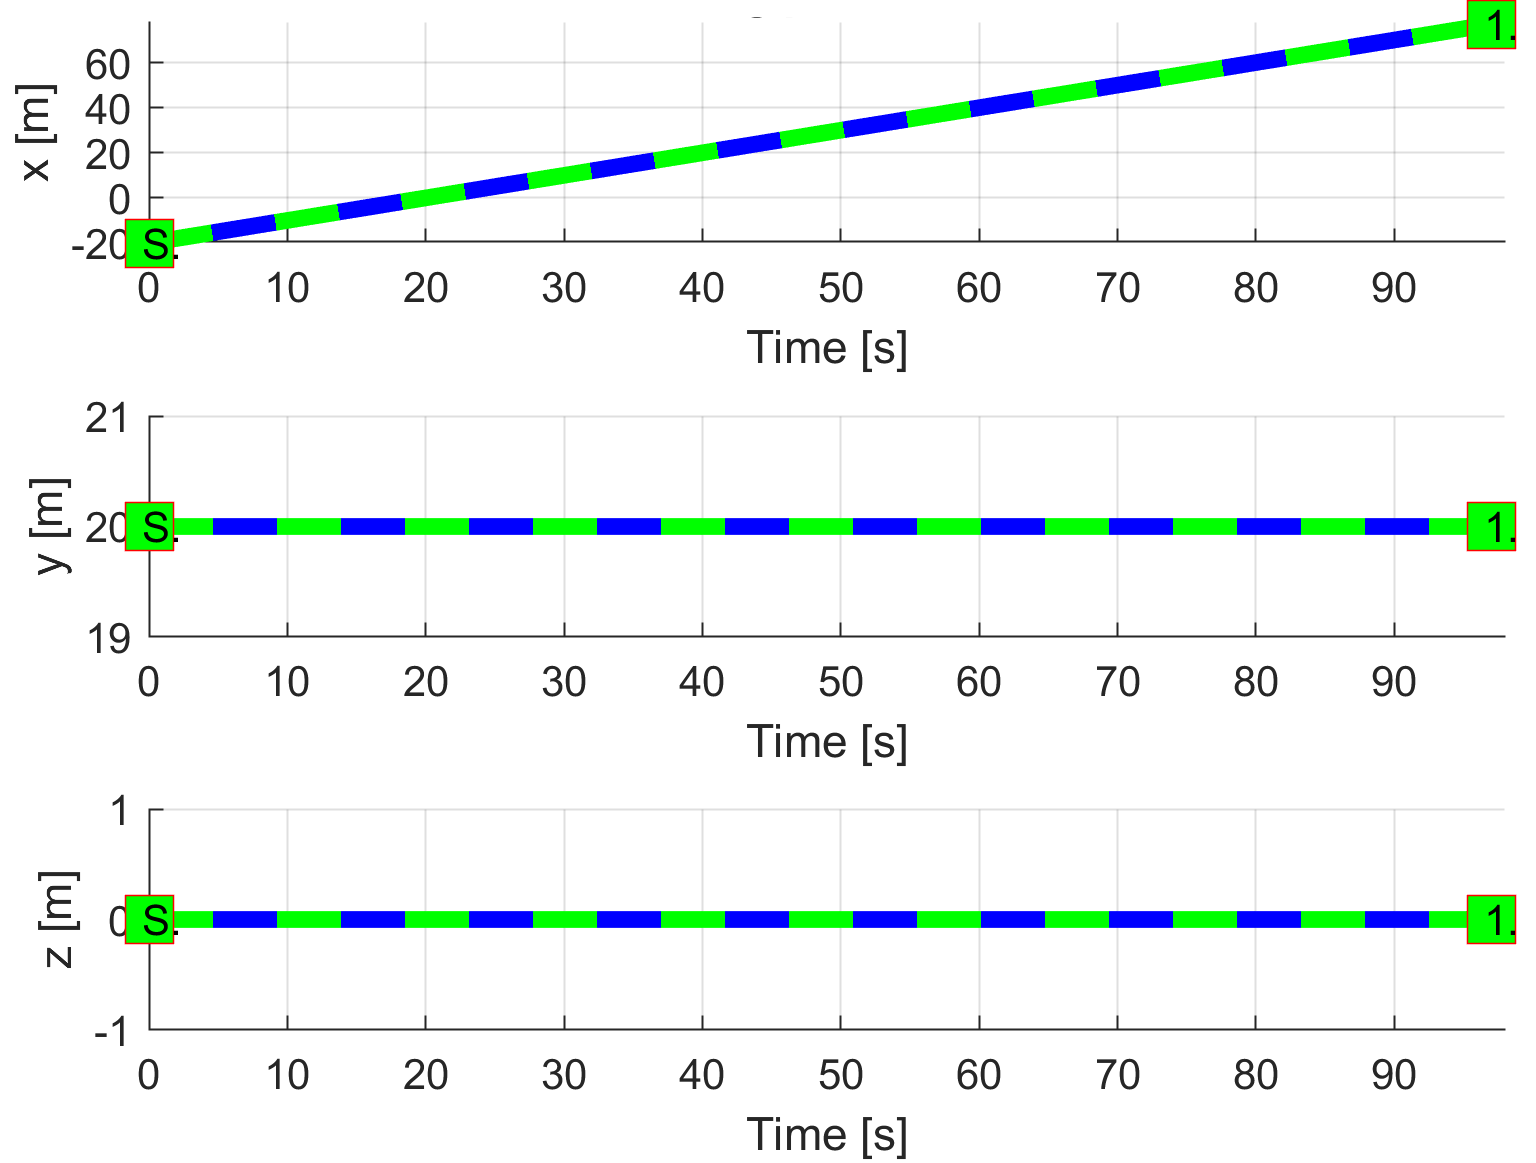
\includegraphics[width=0.9\linewidth]{\FIGDIR/NS077UtmCooperativeOvertake2xSpeedUAV2PathFollowing} 
            \caption{UAS 2.}
            \label{fig:ruleBasedOvertake2xPathTrackingUAS2}
        \end{subfigure}
        \caption{Trajectory tracking for \emph{Rule based overtake double speed} situation test case.}
        \label{fig:testCaseRuleBasedOvertake2xTrajectoryTracking}
    \end{figure}
    
    \paragraph{Path Tracking Deviations: 2x Speed} Path tracking deviations (tab. \ref{tab:pathTrackingParametersForRuleBasedOvertake2x}) are interesting for an \emph{Overtake Maneuver} performance. 
    
    \emph{Maximal deviation distance} is for important waypoints: Divergence ($\mathscr{WP}$ 2.), Convergence ($\mathscr{WP}$ 3.) and Original Goal Waypoint ($\mathscr{WP}$ 4.), equal to $0$ $m$. This is \emph{desired effect} for \emph{Overtake maneuver}.
    
    \emph{Collision point} ($\mathscr{WP}$ 1.) is avoided at minimal distance $5.7991$ $m$ (tab. \ref{tab:testCaseRuleBasedOvertakeSafetyMarginDistancesTimes}) and maximal distance $24.5$ $m$ (tab. \ref{tab:pathTrackingParametersForRuleBasedOvertake2x}). 
    
    Other \emph{Speed Difference Ratios} yields similar results.
    
    \begin{table}[H]
        \centering
        \begin{tabular}{c||c|c|c|c|c}
            \multirow{3}{*}{Param.} & \multicolumn{4}{c|} {UAS 1} & UAS 2     \\\cline{2-6}
                                    & $\mathscr{WP}_1$   & $\mathscr{WP}_2$ & $\mathscr{WP}_3$ & $\mathscr{WP}_4$ & $\mathscr{WP}_1$ \\\cline{2-6}
                                    & col.               & div.             & conv.            & orig.              & nav.              \\\hline\hline
              $\max |x|$            & 20                 & 0                & 0                & 0                & 0                \\\hline
              $\max |y|$            & 6                  & 0                & 4                & 5                & 0                \\\hline
              $\max |z|$            & 0                  & 0                & 0                & 0                & 0                \\\hline
              $\max dist.$          & 24.5                  & 0                & 4                & 5                & 0                \\
        \end{tabular}
        \caption{Path tracking properties for \emph{Rule overtake 2x speed} scenario.}
        \label{tab:pathTrackingParametersForRuleBasedOvertake2x}
    \end{table}


% 11 Rule Based Overtake
\paragraph{Computation Load:} The \emph{computation load} for \emph{scenario} (fig.\ref{fig:ruleBasedOvertakeComputationTime}) shows used time (y-axis) over decision frame (x-axis).

The load is minimal on both UAS, because the rule calculates only divergence (eq. \ref{eq:overtakedDivergenceGlobal}) and convergence (eq. \ref{eq:overtakeConvergenceGlobal}) waypoints.

\begin{figure}[H]
    \centering
    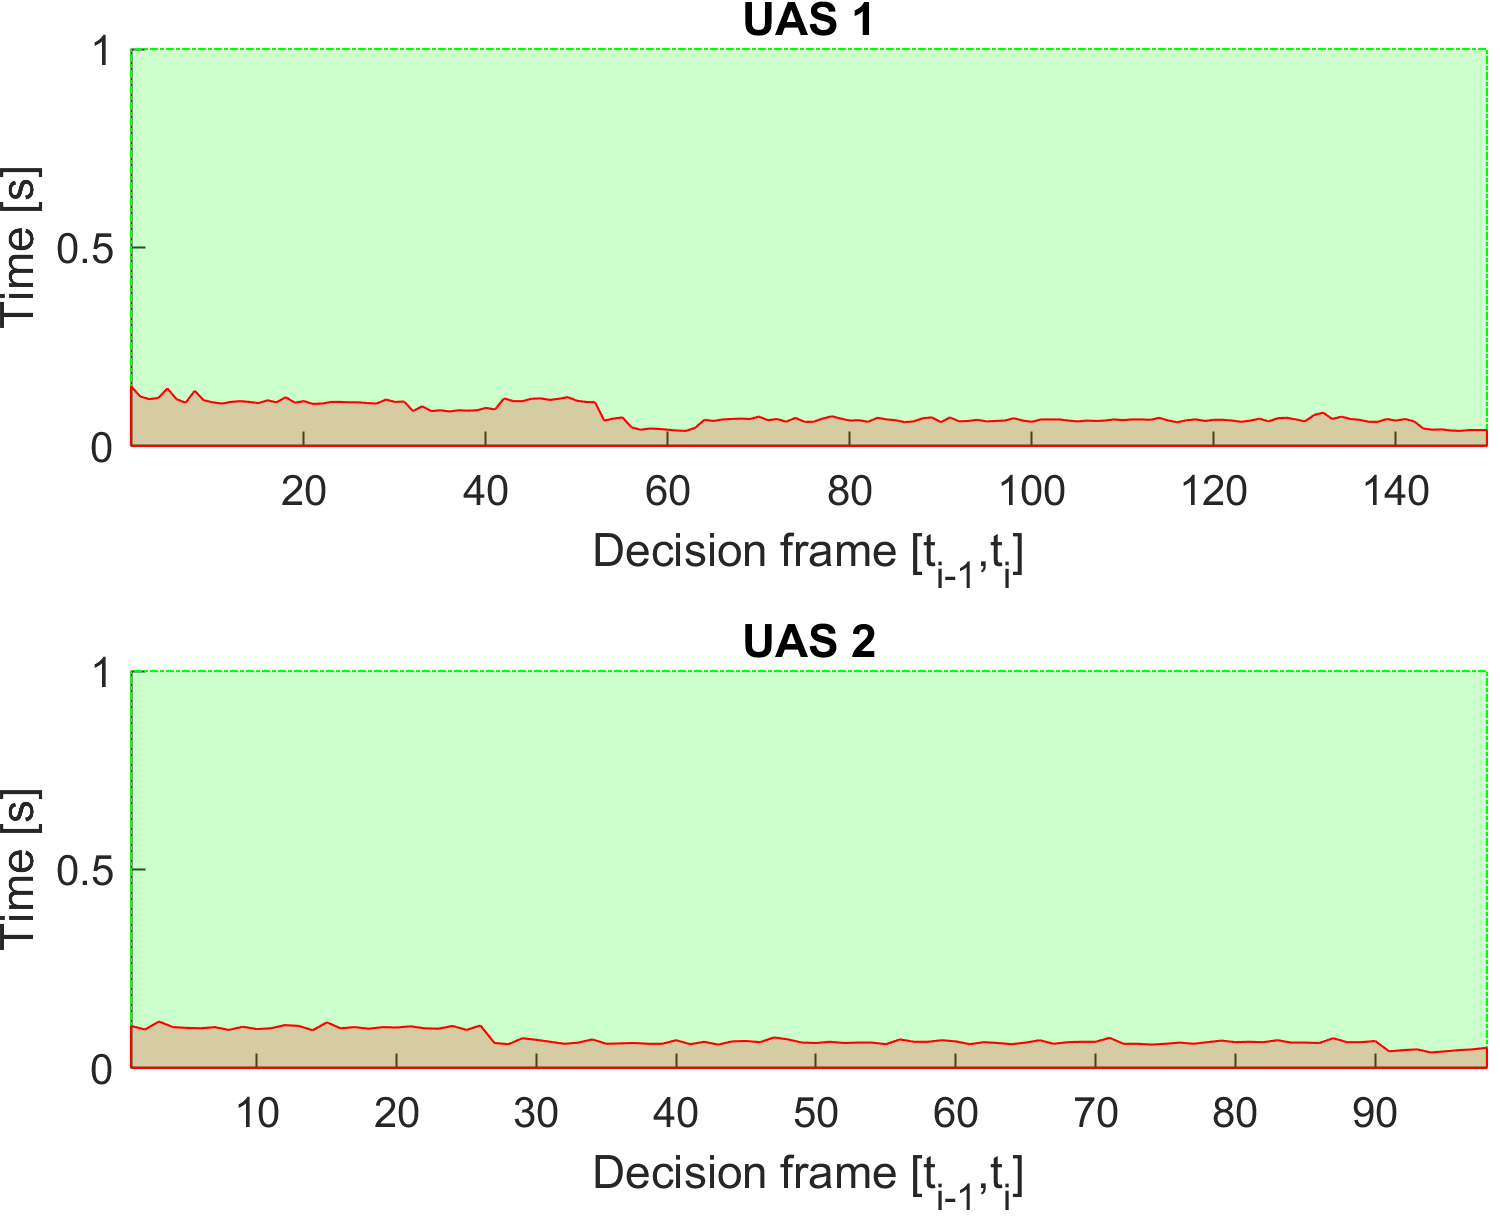
\includegraphics[width=0.65\linewidth]{\FIGDIR/NS102RuleBasedOvertakeComputationTime} 
    \caption{Computation time for \emph{Rule based overtake} scenario.}
    \label{fig:ruleBasedOvertakeComputationTime}
\end{figure}
